\documentclass[a4paper,12pt]{article}

\usepackage{a4wide}
\usepackage{amsfonts}
\usepackage{amsmath}
\usepackage{amssymb}
\usepackage{graphicx}  % For including images
\usepackage{xcolor}  % For a colorfull presentation
\usepackage{listings}  % For presenting code 
\usepackage{hyperref}

\begin{document}
\title{Numerical Optimization \\ Week 1}
\author{Xiaohan Wang gkt918}
\date{11 February}
\maketitle

% \tableofcontents
\section{Brief introduction}
In the first week we reviewed some basics of Linear Algebra, Conditioning and Calculus, and implemented some basic functions using python.
\section{Programming}
\subsection{Function 1}
I have plotted the image of the f1 function in 2D and 3D with the dimension of x being 2 $(-0.1 \leq x_1, x_2 \leq 0.1)$.\\
\begin{figure}[htbp]
\centering
\begin{minipage}[t]{0.48\textwidth}
\centering
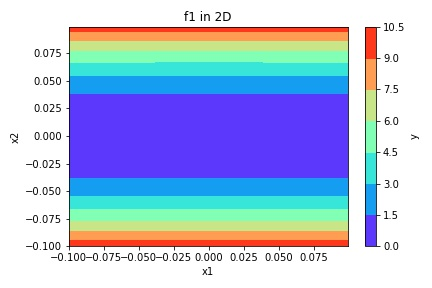
\includegraphics[width=6cm]{f1_2d.jpg}
\caption{f1 in 2D}
\end{minipage}
\begin{minipage}[t]{0.48\textwidth}
\centering
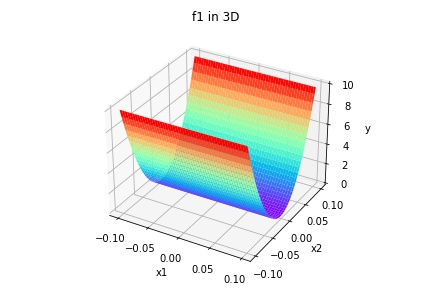
\includegraphics[width=6cm]{f1_3d.jpg}
\caption{f1 in 3D}
\end{minipage}
\end{figure}\\
Its gradient is $2*\alpha^{\frac{i-1}{d-1}}x_i$ for every $x_i$ and Hessian matrix is 
\begin{align*}
H(f_1) = \bigtriangledown^2 f_1(x) = 
\begin{bmatrix}
2*\alpha^{\frac{0}{d-1}} & 0 & \hdots & 0\\
0 & 2*\alpha^{\frac{1}{d-1}} & \hdots & 0 \\
\vdots & \vdots & \ddots & \vdots \\ 
0 & 0 & \hdots & 2*\alpha^{\frac{d-1}{d-1}}
\end{bmatrix}
\end{align*}
I picked 10 points at random and calculated their function values, first and second derivatives through an online calculator. At the same time, I also take these points as input to my implementation and record the value of the output. After comparison, the function value, the first derivative and the second  derivative of each point are the same. So it proves that the function is implemented correctly.




\subsection{Function 2}
I have plotted the image of the f2 function in 2D and 3D $(-0.1 \leq x_1, x_2 \leq 0.1)$.\\
\begin{figure}[htbp]
\centering
\begin{minipage}[t]{0.48\textwidth}
\centering
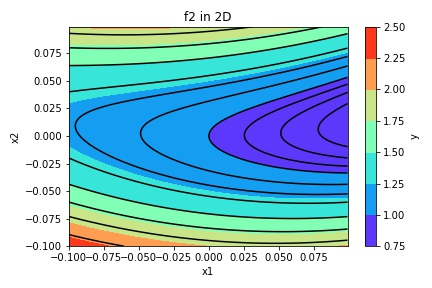
\includegraphics[width=6cm]{f2_2d.jpg}
\caption{f2 in 2D}
\end{minipage}
\begin{minipage}[t]{0.48\textwidth}
\centering
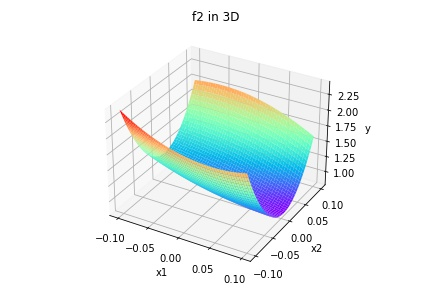
\includegraphics[width=6cm]{f2_3d.jpg}
\caption{f2 in 3D}
\end{minipage}
\end{figure}\\
Its gradient is $(2x_1 - 2 + 400x_1^3 - 400x_1x_2, 200x_2-200x_2^2)$ and Hessian matrix is 
\begin{align*}
H(f_2) = \bigtriangledown^2 f_2(x) = 
\begin{bmatrix}
2+1200x_1^2-400x_2 & -400x_1 \\
-400x_1 & 200
\end{bmatrix}
\end{align*}
The test method is the same as function 1.



\subsection{Function 3}
I have plotted the image of the f3 function in 2D and 3D $(-0.1 \leq x_1, x_2 \leq 0.1)$.\\
\begin{figure}[htbp]
\centering
\begin{minipage}[t]{0.48\textwidth}
\centering
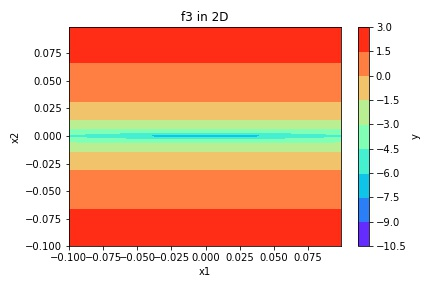
\includegraphics[width=6cm]{f3_2d.jpg}
\caption{f3 in 2D}
\end{minipage}
\begin{minipage}[t]{0.48\textwidth}
\centering
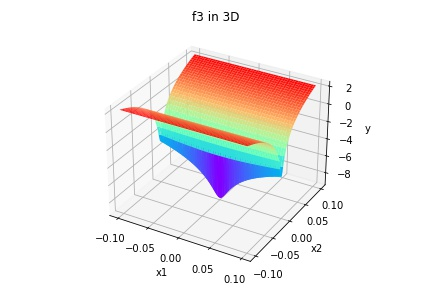
\includegraphics[width=6cm]{f3_3d.jpg}
\caption{f3 in 3D}
\end{minipage}
\end{figure}\\
Its gradient is $\#todo$ and Hessian matrix is 
\begin{align*}
H(f_3) = \bigtriangledown^2 f_3(x) = 
\begin{bmatrix}
\#todo
\end{bmatrix}
\end{align*}
The test method is the same as function 1.


\subsection{Function 4}
I have plotted the image of the f4 function in 2D and 3D $(-0.1 \leq x_1, x_2 \leq 0.1)$.\\
\begin{figure}[htbp]
\centering
\begin{minipage}[t]{0.48\textwidth}
\centering
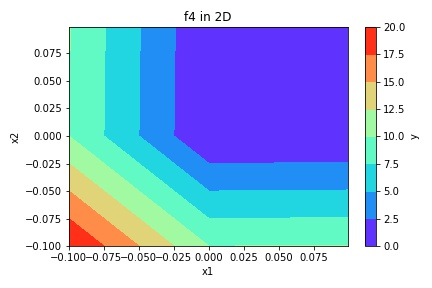
\includegraphics[width=6cm]{f4_2d.jpg}
\caption{f4 in 2D}
\end{minipage}
\begin{minipage}[t]{0.48\textwidth}
\centering
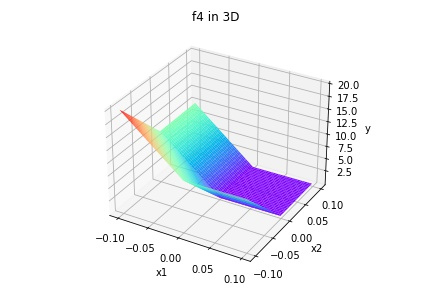
\includegraphics[width=6cm]{f4_3d.jpg}
\caption{f4 in 3D}
\end{minipage}
\end{figure}\\
Its gradient is $\#todo$ and Hessian matrix is 
\begin{align*}
H(f_4) = \bigtriangledown^2 f_4(x) = 
\begin{bmatrix}
\#todo
\end{bmatrix}
\end{align*}
The test method is the same as function 1.
\subsection{Function 5}
I have plotted the image of the f4 function in 2D and 3D $(-0.1 \leq x_1, x_2 \leq 0.1)$.\\
\begin{figure}[htbp]
\centering
\begin{minipage}[t]{0.48\textwidth}
\centering
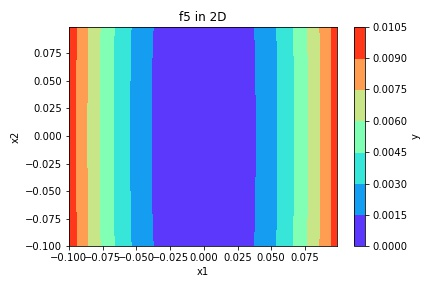
\includegraphics[width=6cm]{f5_2d.jpg}
\caption{f5 in 2D}
\end{minipage}
\begin{minipage}[t]{0.48\textwidth}
\centering
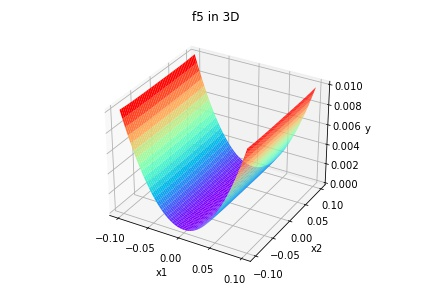
\includegraphics[width=6cm]{f5_3d.jpg}
\caption{f5 in 3D}
\end{minipage}
\end{figure}\\
Its gradient is $\#todo$ and Hessian matrix is 
\begin{align*}
H(f_5) = \bigtriangledown^2 f_5(x) = 
\begin{bmatrix}
\#todo
\end{bmatrix}
\end{align*}
The test method is the same as function 1.



\section{Theoretical Exercises}
\subsection{Question 1}
We know the Hessian of f is :
\begin{align*}
H(f) = \bigtriangledown^2 f(x) = 
\begin{bmatrix}
\frac{\partial^2 f}{\partial x_1^2} & \frac{\partial^2 f}{\partial x_1x_2} & \hdots & \frac{\partial^2 f}{\partial x_1x_N}\\
\frac{\partial^2 f}{\partial x_2x_1} & \frac{\partial^2 f}{\partial x_2^2} & \hdots & \frac{\partial^2 f}{\partial x_2x_N} \\
\vdots & \vdots & \ddots & \vdots \\ 
\frac{\partial^2 f}{\partial x_Nx_1} & \frac{\partial^2 f}{\partial x_Nx_2} & \hdots & \frac{\partial^2 f}{\partial x_N^2}
\end{bmatrix}
\end{align*}
Besides, $f(x)=\sum^N_{i=1}g_i(x_i)$, $x \in \mathbb{R}^N$. And it is easy to prove that for $i \neq j$, $\frac{\partial}{\partial x_j} g_i(x_i) = 0$, $\frac{\partial}{\partial x_j} g_i^{'}(x_i) = 0$. Therefore we have
\begin{align*}
\frac{\partial^2 f}{\partial x_ix_j} &= \frac{\partial}{\partial x_j}[\frac{\partial}{\partial x_i} [ g_1(x_1)+g_2(x_2)+...+g_N(x_N) ]]\\
&= \frac{\partial}{\partial x_j}[\frac{\partial}{\partial x_i}g_1(x_1)+\frac{\partial}{\partial x_i}g_2(x_2)+...+\frac{\partial}{\partial x_i}g_N(x_N)] \\
&= \frac{\partial}{\partial x_j}[0 + 0 + \dots + g_i^{'}(x_i)] = 0
\end{align*}
\begin{align*}
\frac{\partial^2 f}{\partial x_i^2} &= \frac{\partial}{\partial x_i}[\frac{\partial}{\partial x_i} [ g_1(x_1)+g_2(x_2)+...+g_N(x_N) ]]\\
&= \frac{\partial}{\partial x_i}[\frac{\partial}{\partial x_i}g_1(x_1)+\frac{\partial}{\partial x_i}g_2(x_2)+...+\frac{\partial}{\partial x_i}g_N(x_N)] \\
&= \frac{\partial}{\partial x_i}[0 + 0 + \dots + g_i^{'}(x_i)] = g_i^{''}(x_i)
\end{align*}
Now, we have 
\begin{align*}
H(f) = \bigtriangledown^2 f(x) = 
\begin{bmatrix}
g_1^{''}(x_1) & 0 & \hdots & 0\\
0 & g_2^{''}(x_2) & \hdots & 0 \\
\vdots & \vdots & \ddots & \vdots \\ 
0 & 0 & \hdots & g_N^{''}(x_N)
\end{bmatrix}
\end{align*}
It means that $(\bigtriangledown^2 f(x))_{ii} = g_i^{''}(x_i)$.


\subsection{Question 3}
At $x = (1,1)$ point, $f_3(x)^{'} = 0$ and  $f_3(x)^{''} < 0$. Therefore, point (1,1) is a minimizer.
\subsection{Question 4}
From the question, we know that we should prove log(1 + exp(x)) = log(1 + exp(-|x|)) + max(x, 0), which can be rewritten as 
\begin{align*}
&log(1 + e^x) - log(1 + e^{-|x|}) - max(x, 0) = 0\\
\Rightarrow &\ log\frac{1 + e^x}{1 + e^{-|x|}} - max(x, 0) = 0
\end{align*}
When $x \leq 0$, we have $-|x| = x$, $max(x, 0) = 0$, then
\begin{align*}
&log(1 + e^x) - log(1 + e^{-|x|}) - max(x, 0) \\
=&\ log\frac{1 + e^x}{1 + e^{x}} = log1 = 0
\end{align*}
When $x > 0$, we have $-|x| = -x$, $max(x, 0) = x$, then
\begin{align*}
&log(1 + e^x) - log(1 + e^{-|x|}) - max(x, 0) \\
=&\ log\frac{1 + e^x}{1 + e^{-x}}  - x = log\frac{1 + e^x}{1 + e^{-x}}  - log(e^x) \\
=&\ log\frac{1 + e^x}{e^x(1 + e^{-x})} = log\frac{1 + e^x}{1 + e^x} = log1 = 0\\
\end{align*}
Therefore, we have 
\begin{align*}
log(1 + e^x) = log(1 + e^{-|x|}) + max(x, 0)
\end{align*}
Otherwise, if we use $log(1 + e^x)$ to calculate the floating-point in f4, When $x \leq 0$ they have no difference. But when $x > 0$, it is easy to lose precision, because $e^x$ enlarges $x$ to a large number, and then reduces it to another number through $log$. In this process, the precision will be inaccurate due to multiple operations.\\
On the other hand, $log(1 + e^{-|x|}) + max(x, 0)$ can maintain the accuracy better because the $x$ is taken out separately.\\
At the same time, when $x$ is very large, $e^x$ may be too large to calculate, while $e^{-|x|}$ will not.
\section{Conclusion}
From this assignment, I have a certain grasp of the basic theory of the course, and at the same time, I have completed the programming of functions, laying a foundation for future study.
\end{document}